\chapter{Docker}
\label{Docker}
\thispagestyle{plain}

Docker \cite{docker} è una piattaforma per sviluppare, spedire e avviare applicazioni usando la tecnologia dei container. Il progresso dell'industria tecnologica procede ad un ritmo elevatissimo e sempre più aziende hanno bisogno di strumenti affidabili e facilmente scalabili a seconda delle esigenze. La piattaforma Docker è lo strumento all'avanguardia che permette la consegna ed installazione di servizi in semplicità e sicurezza, mediante componenti leggeri e standard, assai portabili e aggiornabili, chiamati \emph{container}. Questi non solo sono utilizzati per sviluppare nuovi servizi e micro-servizi, ma anche per eseguire applicazioni esistenti, preparandole ad una futura modernizzazione. I vantaggi della piattaforma hanno convinto l'industria, che oggi confida sempre più su questa tecnologia, costruendo piattaforme di container.

\section{Versioni}
Docker è un software disponibile per diversi sistemi operativi fra cui sistemi Linux (Ubuntu, Fedora, Debian, CentOS), Windows, Mac, ma anche in cloud (Amazon Web Services, Microsoft Azure). È disponibile in due versioni:
\begin{itemize}
    \item Community Edition (CE): gratuita, ideale per sviluppatori singoli e per piccoli team. Possiede le funzionalità di base della piattaforma.
    \item Enterprise Edition (EE): studiata per sviluppo aziendale e per team che sviluppano, spediscono ed eseguono applicazioni essenziali per l'impresa.
\end{itemize}

\section{Architettura, componenti e funzionamento}
Docker \cite{docker_doc} utilizza funzionalità di virtualizzazione del kernel Linux per avviare servizi e applicazioni in un ambiente isolato, protetto e sicuro. In seguito si descriveranno i componenti base di Docker e come interagiscono fra loro.

\subsection{Immagini}
Un'immagine è un template con istruzioni per la creazione di container. Le immagini descrivono anche i componenti e i programmi all'interno del container e possono includere anche altre immagini. Ad esempio, è possibile indicare che sull'immagine "Ubuntu" sia installato il web server Apache ed altre applicazioni con le relative impostazioni. È possibile creare le proprie immagini, ma anche utilizzarne altre disponibili su \hyperref[docker-hub]{Docker Hub}. Per creare un immagine è necessario creare un \emph{Dockerfile} che indichi gli step per la creazione e l'avvio dell'immagine. Ogni step costituisce un layer dell'immagine: la ricreazione dell'immagine a fronte di modifiche comporterà la sola sostituzione dei layer modificati. L'operazione risulta quindi assai conveniente, leggera e veloce.

\subsection{Container}
Un container è un'istanza eseguibile di un'immagine. Ogni container possiede i propri processi, la propria memoria, i propri dispositivi e stack di rete. I container isolano quindi il proprio ambiente da quello esterno, assicurandosi che i propri applicativi funzionino sempre e in modo sicuro, indipendentemente dalle specifiche dell'host. È possibile connettere un container alla rete oppure ad altri container, assegnargli spazio di archiviazione e utilizzare lo stato attuale per creare nuove immagini. Pertanto un container è definito dalla sua immagine e dalla sua configurazione di avvio. Al riavvio di un container, ogni modifica apportata al suo stato o ai suoi dati verrà persa. È possibile introdurre la persistenza dei dati utilizzando la tecnologia dei \emph{volumi}. Questi sono completamente gestiti da Docker, sono facili da eseguire o migrare e sono utilizzabili in sicurezza da più container. La creazione di un volume consiste nella copia di una directory dal filesystem del container verso il filesystem dell'host. Docker gestisce direttamente il contenuto di queste directory. Ad esempio, a seguito del riavvio di un container, Docker carica i dati salvati sull'host all'interno della directory specificata, ripristinando il suo stato prima dello spegnimento.

\subsection{Docker Engine}
Docker Engine è un'applicazione con architettura di tipo client-server. È costituita da tre componenti:
\begin{itemize}
    \item Un processo daemon (\verb|dockerd|) che rappresenta il server.
    \item Una REST API che definisce in che modo i programmi possono interagire con il processo daemon.
    \item Un'interfaccia a linea di comando (\verb|docker|) che rappresenta il client.
\end{itemize}
Il daemon riceve richieste dal client per costruire, eseguire e distribuire container e può comunicare con altri daemon per gestire servizi Docker più complessi. Il client invece, eseguendo comandi come \verb|docker run|, utilizza le REST API, socket UNIX o interfacce di rete per comunicare col daemon. Client e server possono essere eseguiti sullo stesso host oppure su macchine differenti. Il daemon può gestire richieste differenti: ad esempio \verb|docker pull| ordina al server di collegarsi a \hyperref[docker-hub]{Docker Hub} per scaricare l'immagine di Redis, mentre \verb|docker run| richiede che l'immagine di Ubuntu, già disponibile localmente, sia avviata.
\begin{figure}[h]
    \begin{subfigure}{0.4\textwidth}
        \centering
        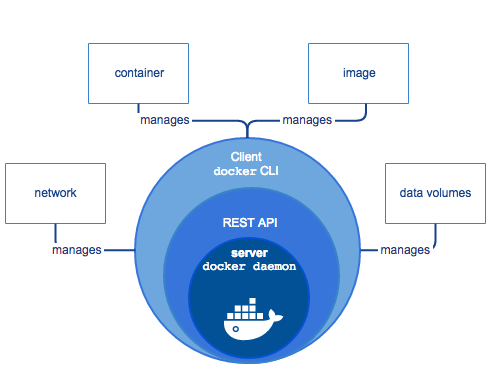
\includegraphics[width=\textwidth]{immagini/engine-components-flow.png}
        \caption{Struttura del Docker Engine}
        \label{fig:docker_engine_a}
    \end{subfigure}
    \begin{subfigure}{0.6\textwidth}
        \centering
        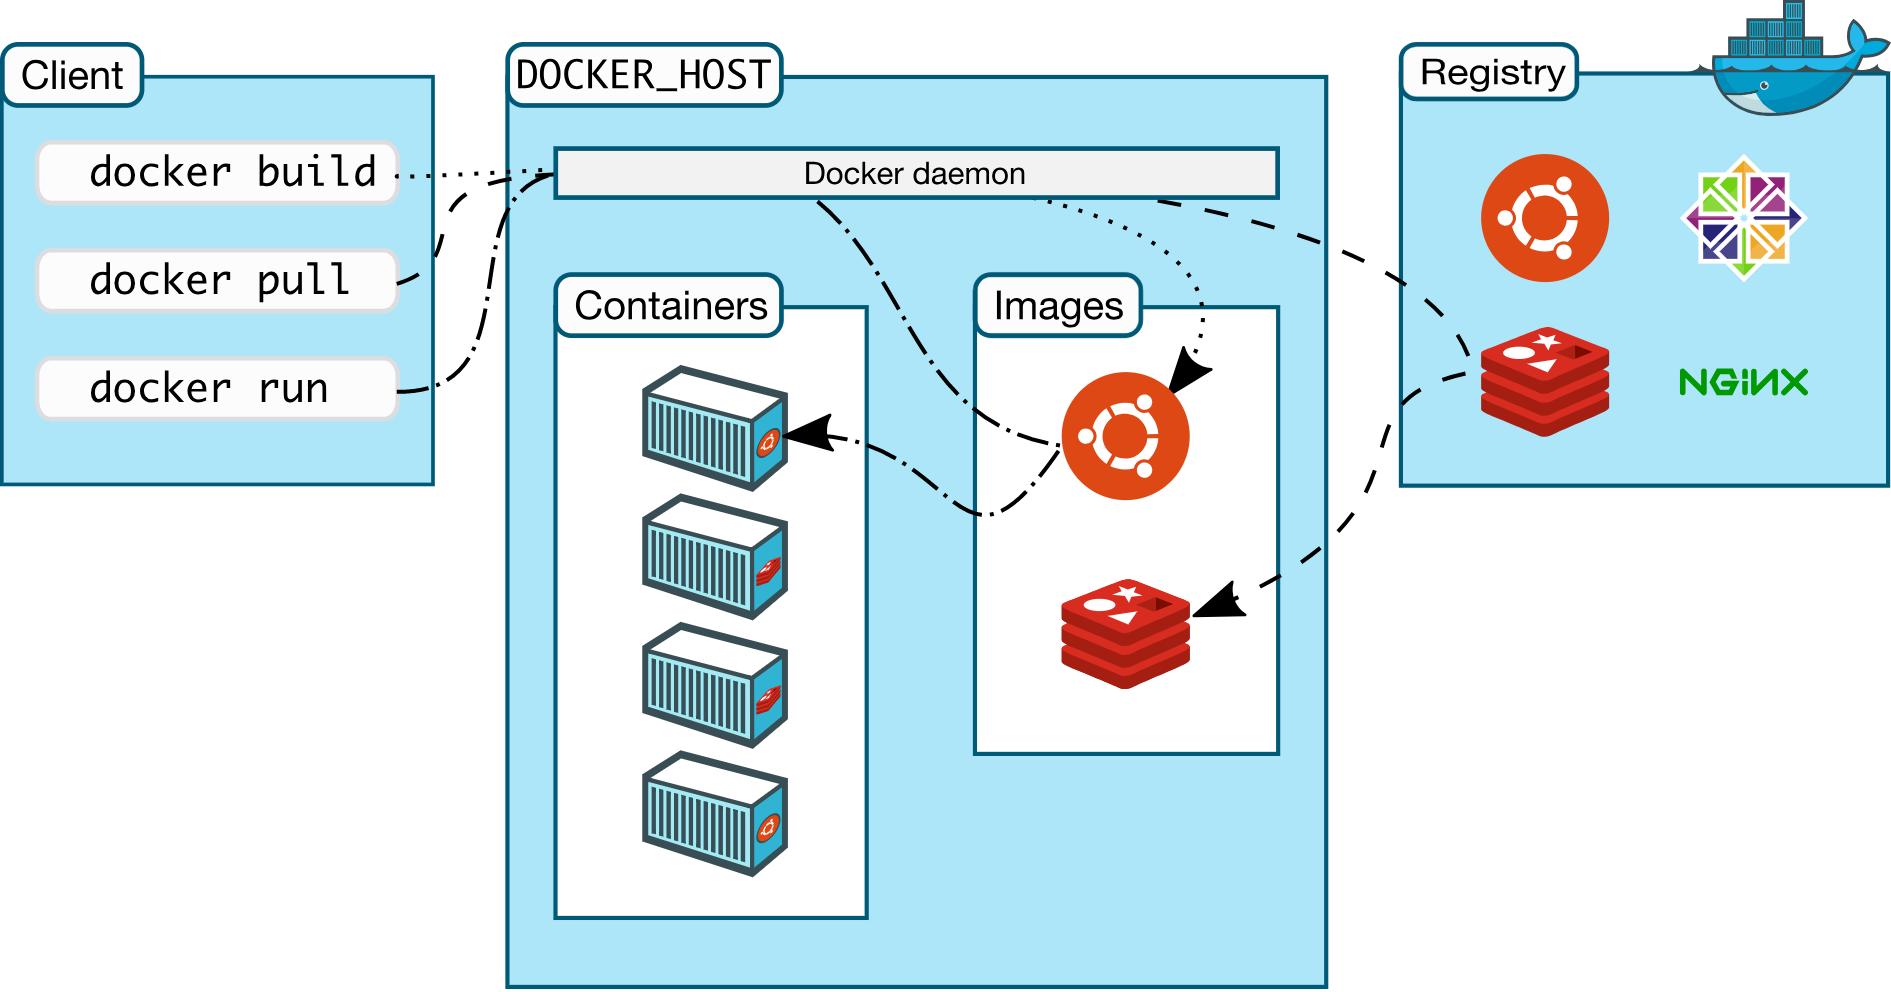
\includegraphics[width=\textwidth]{immagini/architecture.png}
        \caption{Esempio funzionamento Docker Engine}
        \label{fig:docker_engine_b}
    \end{subfigure}
    \caption{Docker Engine}
    \label{fig:docker_engine}
\end{figure}

\subsection{Docker Hub}\label{docker-hub}
Docker Hub è un servizio che consente di collegarsi a repository di immagini, permettendo agli utenti di caricare e scaricare liberamente immagini di container da avviare sui propri host. Costituisce inoltre il nodo centrale per lo sviluppo, la distribuzione e gestione delle modifiche dei container. Docker Hub contiene un gran numero di repository ufficiali, pubblici e certificati dai fornitori. Fra questi si citano NGINX, Redis, MongoDB, Ubuntu, PostgreSQL, Node.js, MySQL, Tomcat e molti altri.

\subsection{Docker Compose}
Docker Compose è uno strumento per definire ed avviare servizi multi-container mediante un file YAML chiamato \verb|docker-compose.yml|. In questo file sono contenute tutte le informazioni per la configurazione dei vari servizi. Attraverso i diversi campi messi a disposizione dal file di configurazione è possibile cambiare il comportamento del container, ad esempio indicando l'immagine o il Dockerfile di riferimento, creando dipendenze da altri servizi, associandogli un numero di porta, indicando comandi da eseguire all'avvio e molto altro. Con lo stesso file si possono gestire più container, le loro dipendenze e avviarli in contemporanea. Pertanto Docker Compose risulta uno strumento utile sia in fase di sviluppo, dove può essere utilizzato per creare ambienti controllati con cui interagire facilmente e testare la propria applicazione, che in fase di distribuzione, quando non è più richiesto all'installatore di preparare l'ambiente per l'applicazione, ma solo di eseguire il comando \verb|docker-compose up|.

Segue un estratto di \verb|docker-compose.yml| utilizzato per il progetto:
\lstinputlisting[lastline=17, caption={Esempio di docker-compose.yml}, captionpos=b, label={esempio_dcyml}]{script/docker-compose.yml}
Nell'esempio (\hyperref[esempio_dcyml]{Codice: 3.1}) è indicata la versione del formato del file, seguita dai servizi da gestire. Con il parametro \verb|restart: always| si impone che in caso di errore del container ShareLaTex venga riavviato. A seguire si specifica il nome dell'immagine di riferimento, il nome del container che verrà creato, le dipendenze, la priorità del container sugli altri, il numero di porta, i collegamenti con altri container e, infine, i volumi da montare sull'host per la persistenza dei dati.
 
\section{Tecnologia sottostante}
Docker è scritto in linguaggio GO ed utilizza diverse funzionalità del kernel Linux per eseguire container in ambienti controllati, in modo leggero e veloce. Tali funzionalità sono raccolte all'interno della libreria \emph{libcontainer}, che permette a Docker Engine di gestire il ciclo di vita dei container.

\subsection{Namespace}
Docker Engine utilizza la tecnologia dei \emph{namespace} per creare un gruppo di namespace all'avvio di ogni container. In tal modo ad ogni container è associato un ambiente isolato, ottenuto come risultato di una partizione delle risorse del kernel host. Pertanto i namespace limitano ciò che un container vede e quindi può utilizzare. I namespace utilizzati in Docker sono:
\begin{itemize}
    \item PID: per isolare i processi appartenenti ad un determinato container da quelli in esecuzione sull'host o in altri container.
    \item NET: per la gestione delle interfacce di rete.
    \item IPC: per la gestire gli accessi alle risorse di Inter Process Communication.
    \item MNT: per gestire i punti di mount del filesystem.
    \item UTS: per dare a ogni container un hostname.
\end{itemize}
%È importante sottolineare che ogni processo è in un namespace di ogni tipo. Ad esempio, processi con un un certo PID namespace possono vedere solo processi nello stesso PID namespace.

\subsection{Cgroup}
Docker Engine utilizza un'altra tecnologia chiamata \emph{cgroup}, ovvero control group, per limitare la quantità di risorse utilizzate da un container. Infatti, le risorse hardware dell'host sono limitate e devono essere ripartite e condivise fra i container, impostando limiti e vincoli di utilizzo. Cgroup dà la possibilità di limitare le risorse (si pensi alla memoria), definire priorità, misurare le risorse utilizzate e controllare processi qualora superino i limiti imposti, congelandoli e riavviandoli quando possibile.

\subsection{Union filesystem}
Union filesystem, anche detto UnionFS, è una tecnologia che consente la sovrapposizione di filesystem separati, ovvero l'aggregazione di file e directory differenti e separate per formare un singolo filesystem. Docker Engine utilizza questa tecnologia per costruire container senza duplicare file o directory. Inoltre, UnionFS permette la scrittura anche su file che appaiono read-only mediante il meccanismo copy-on-write. Si ipotizzi di voler avviare più container con la stessa immagine: in memoria sarebbero presenti tante copie dei filesystem quanti sono i container avviati. Con il meccanismo copy-on-write, il filesystem utilizzato è uno, mentre tutte le modifiche apportate da ogni container risultano salvate su layer copy-on-write di dimensioni contenute. Questo spiega anche come sia possibile, una volta scritto sul filesystem di un container, avviare un secondo container dalla stessa immagine senza conservare le modifiche apportate al primo.

\subsection{Funzionamento su Windows e MacOS}
Le tecnologie precedentemente elencate sono proprie del kernel Linux. Le versioni di Docker per Windows e MacOS necessitano di un livello aggiuntivo per avviare container. In Windows è avviata una macchina virtuale Linux leggera tramite Hyper-V, mentre MacOS utilizza HyperKit per lo stesso fine. Tutti i container avviati condivideranno la stessa macchina virtuale su Hyper-V per Windows o su HyperKit per MacOS.

\section{Vantaggi rispetto alla virtualizzazione}
Avviare un servizio in uno o più container piuttosto che all'interno di una o più macchine virtuali risulta conveniente sia in termini di risorse utilizzate, che in termini di facilità di installazione. Gruppi di container sulla stessa macchina condividono il kernel del sistema operativo dell'host, mentre più macchine virtuali necessitano ciascuna di un layer di sistema operativo guest. I container sono quindi più leggeri, non richiedono l'installazione di un sistema operativo e utilizzano meno risorse (RAM, CPU, spazio d'archiviazione) grazie ai meccanismi precedentemente descritti. Inoltre, l'installazione di un servizio all'interno di una macchina virtuale può richiedere impegno nell'installazione dei vari componenti. Questo problema è risolto dai container, che possono essere avviati in un ambiente controllato, installati e gestiti facilmente (si pensi a Docker Compose). Dunque la tecnologia dei container è maggiormente portabile rispetto a quella delle macchine virtuali.
\begin{figure}[h]
    \centering
    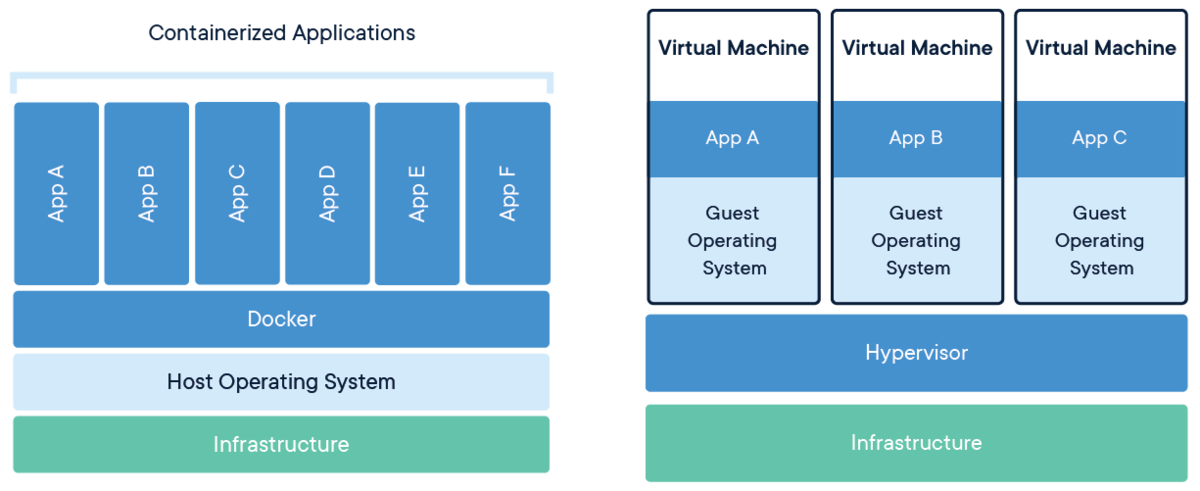
\includegraphics[width=\textwidth]{immagini/docker-containerized-and-vm-transparent-bg.png}
    \caption{Stratificazione di un sistema a container e di un sistema con VMs}
    \label{fig:container-vs-VM}
\end{figure}